
\begin{figure}[h]
    \centering
    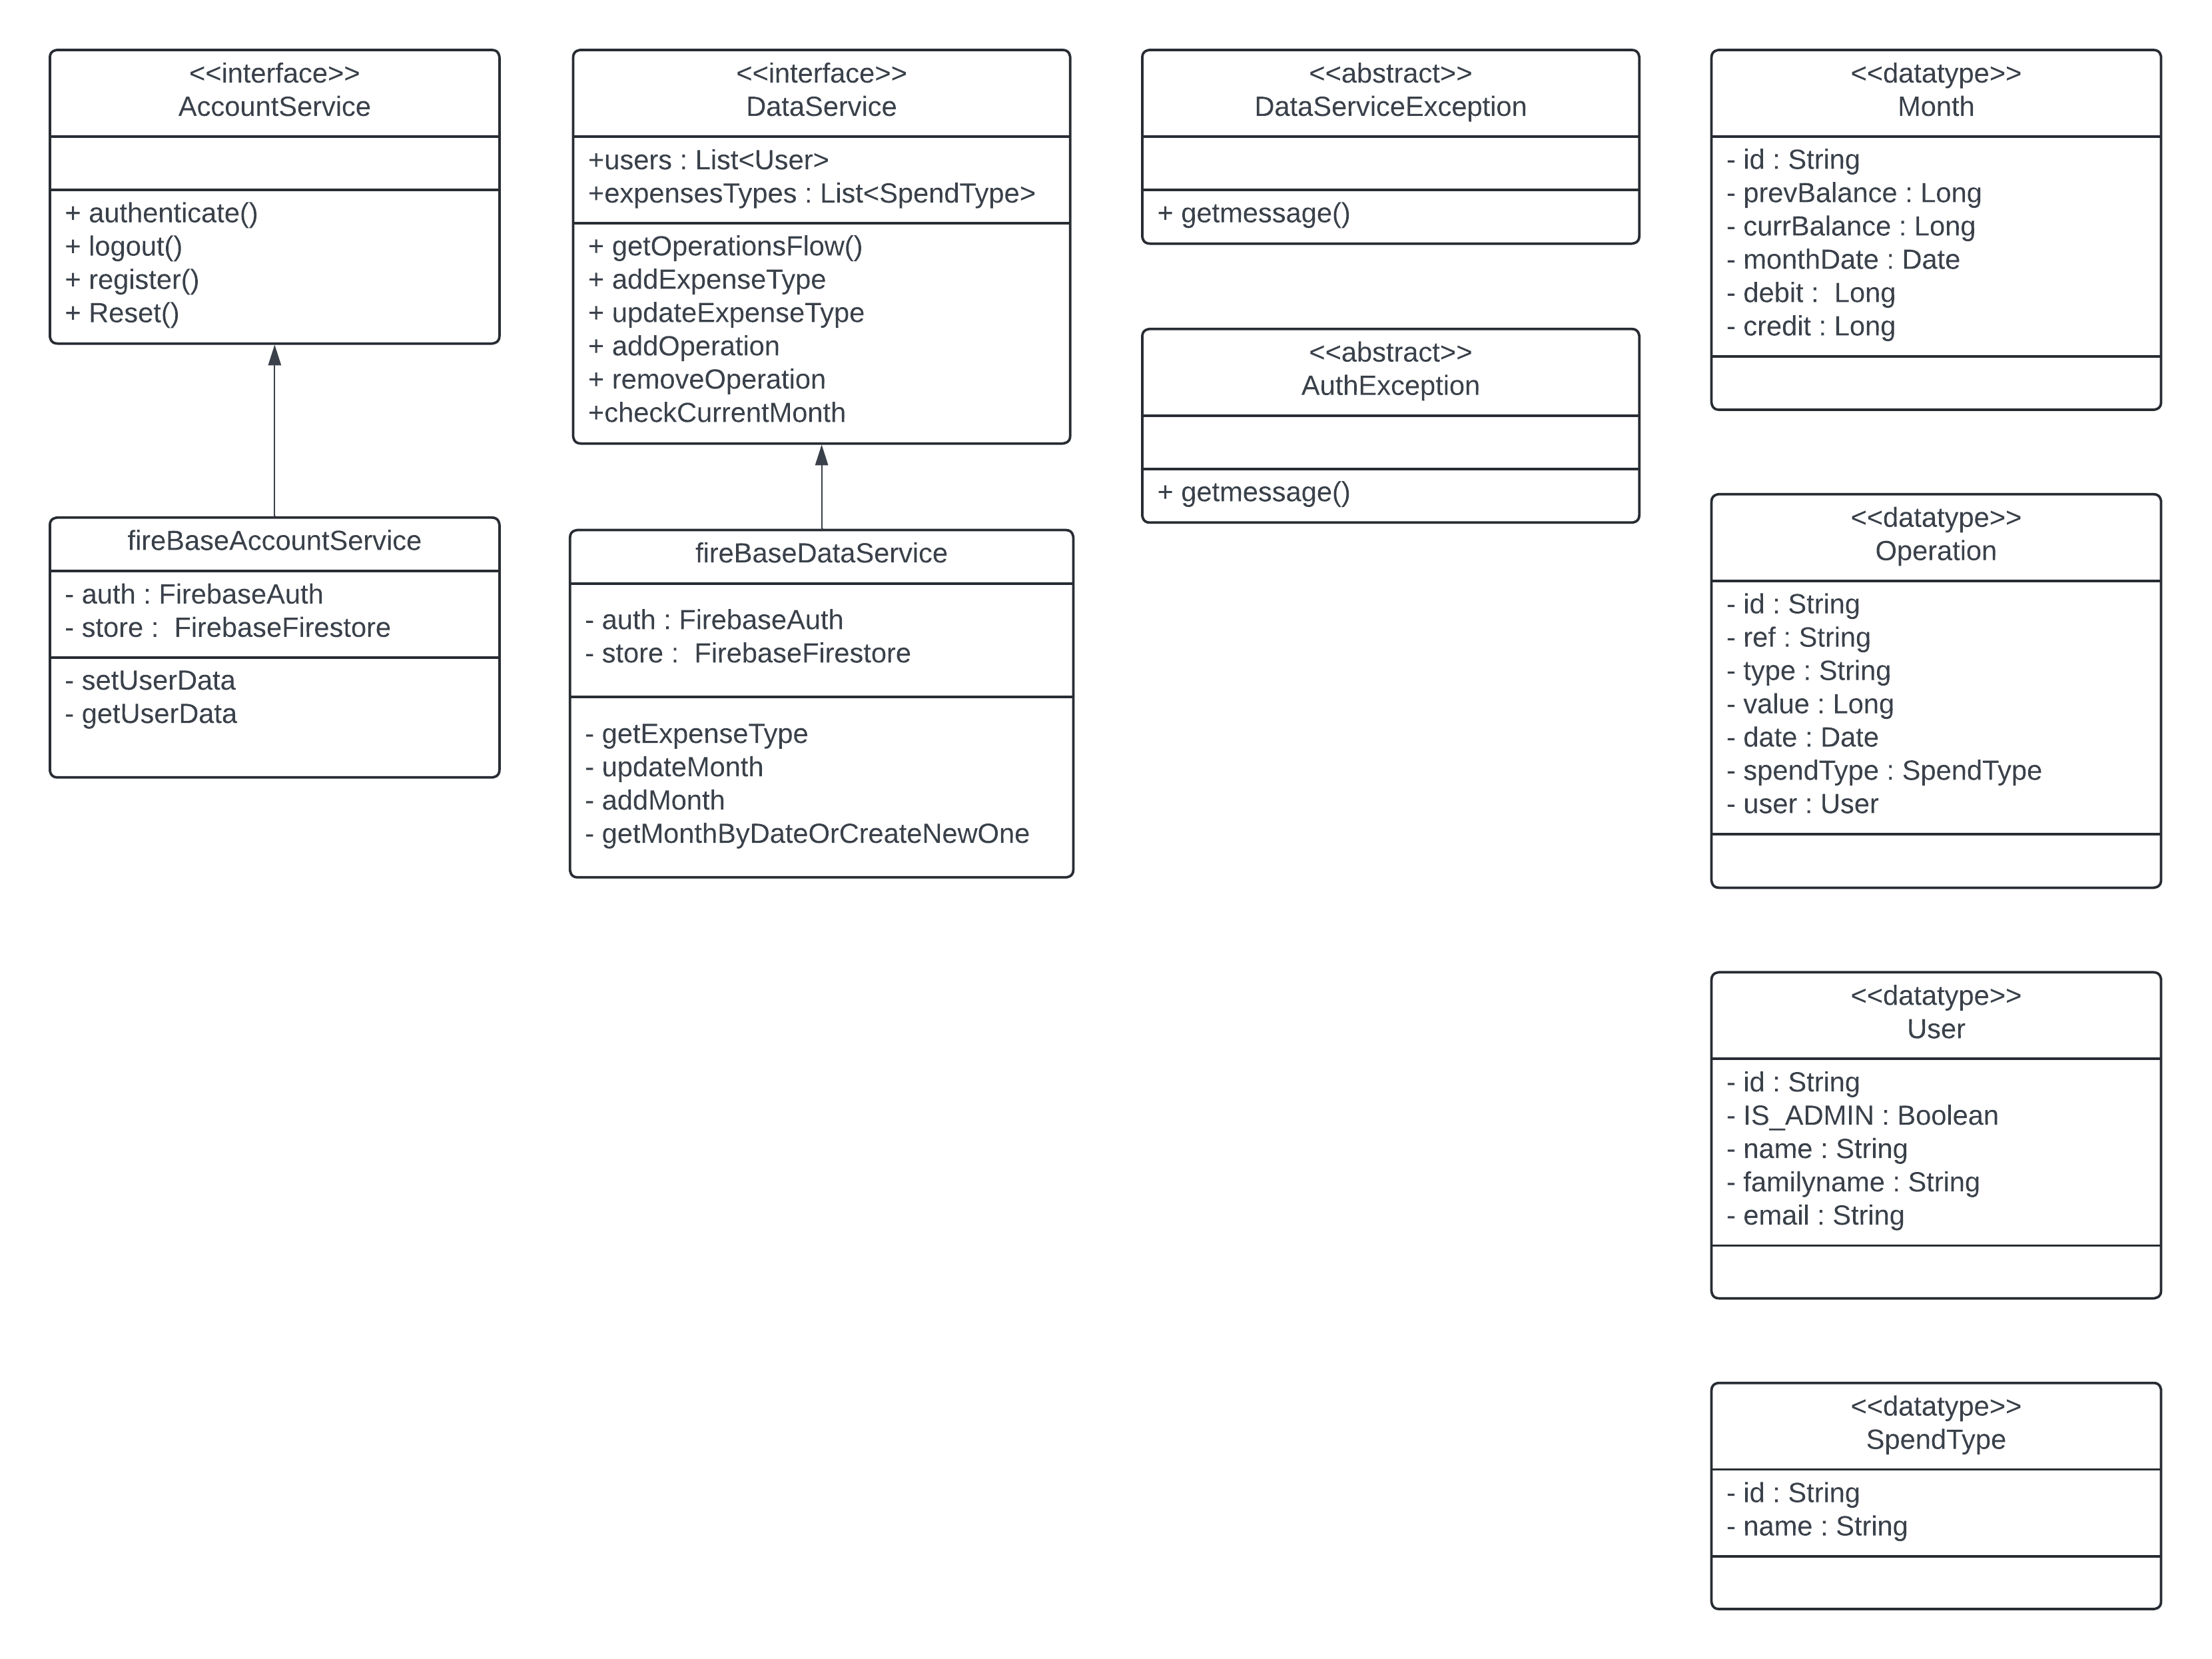
\includegraphics[width=1\textwidth]{diag classe metier.png}
    \caption{Diagramme de classe métier}
\end{figure}


list des products backlog

\begin{figure}[h]
    \centering
    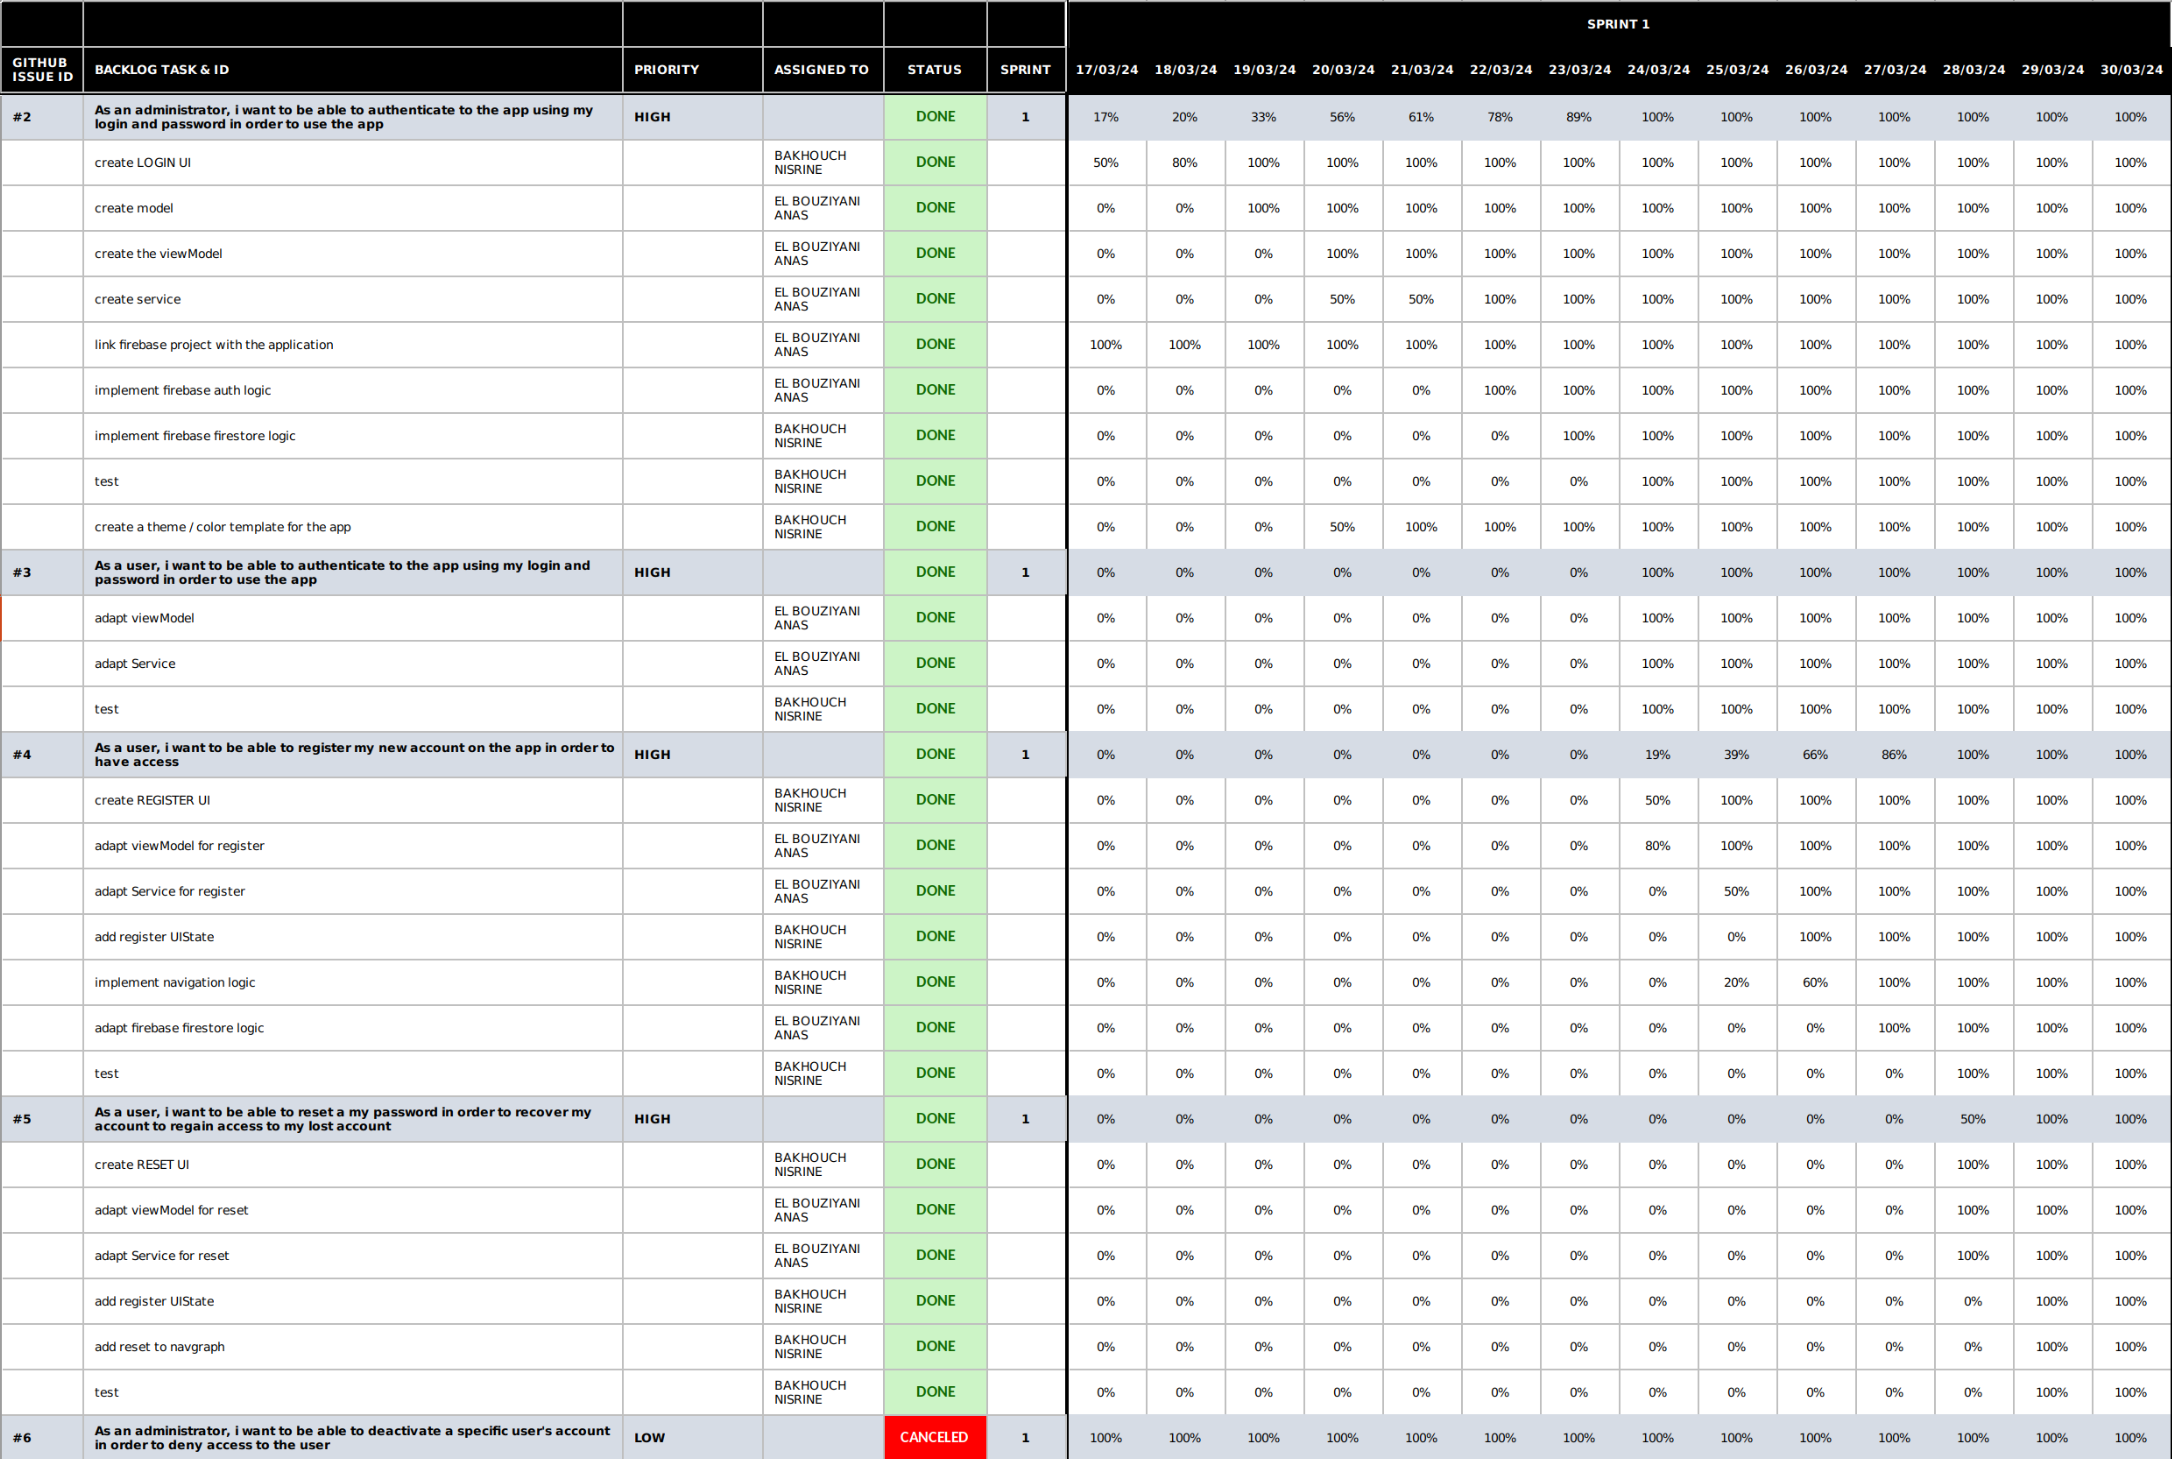
\includegraphics[width=1\textwidth]{sprint1.png}
    \label{Sprint1}
    \caption{Product Backlog de sprint 1}
\end{figure}


\begin{figure}[h]
    \centering
    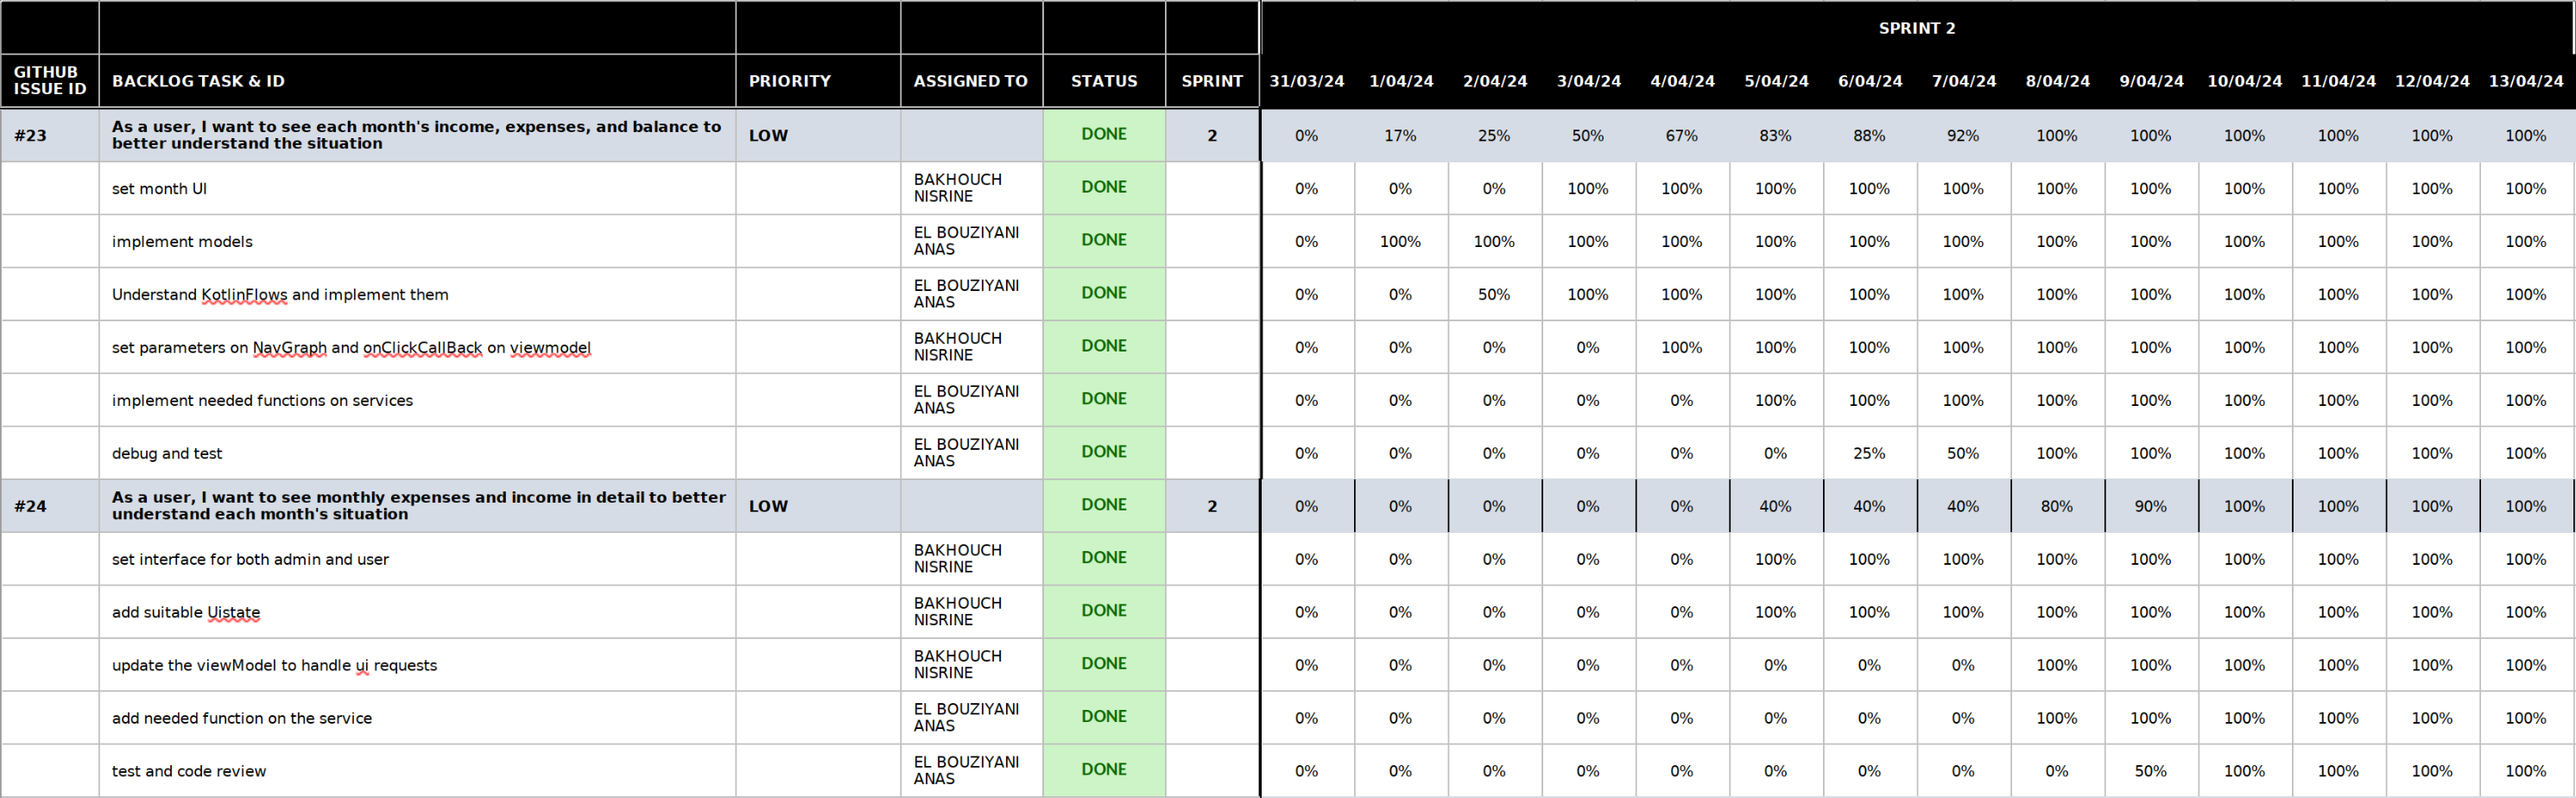
\includegraphics[width=1\textwidth]{sprint2.png}
    \label{Sprint2}
    \caption{Product Backlog de sprint 2}
\end{figure}


\begin{figure}[h]
    \centering
    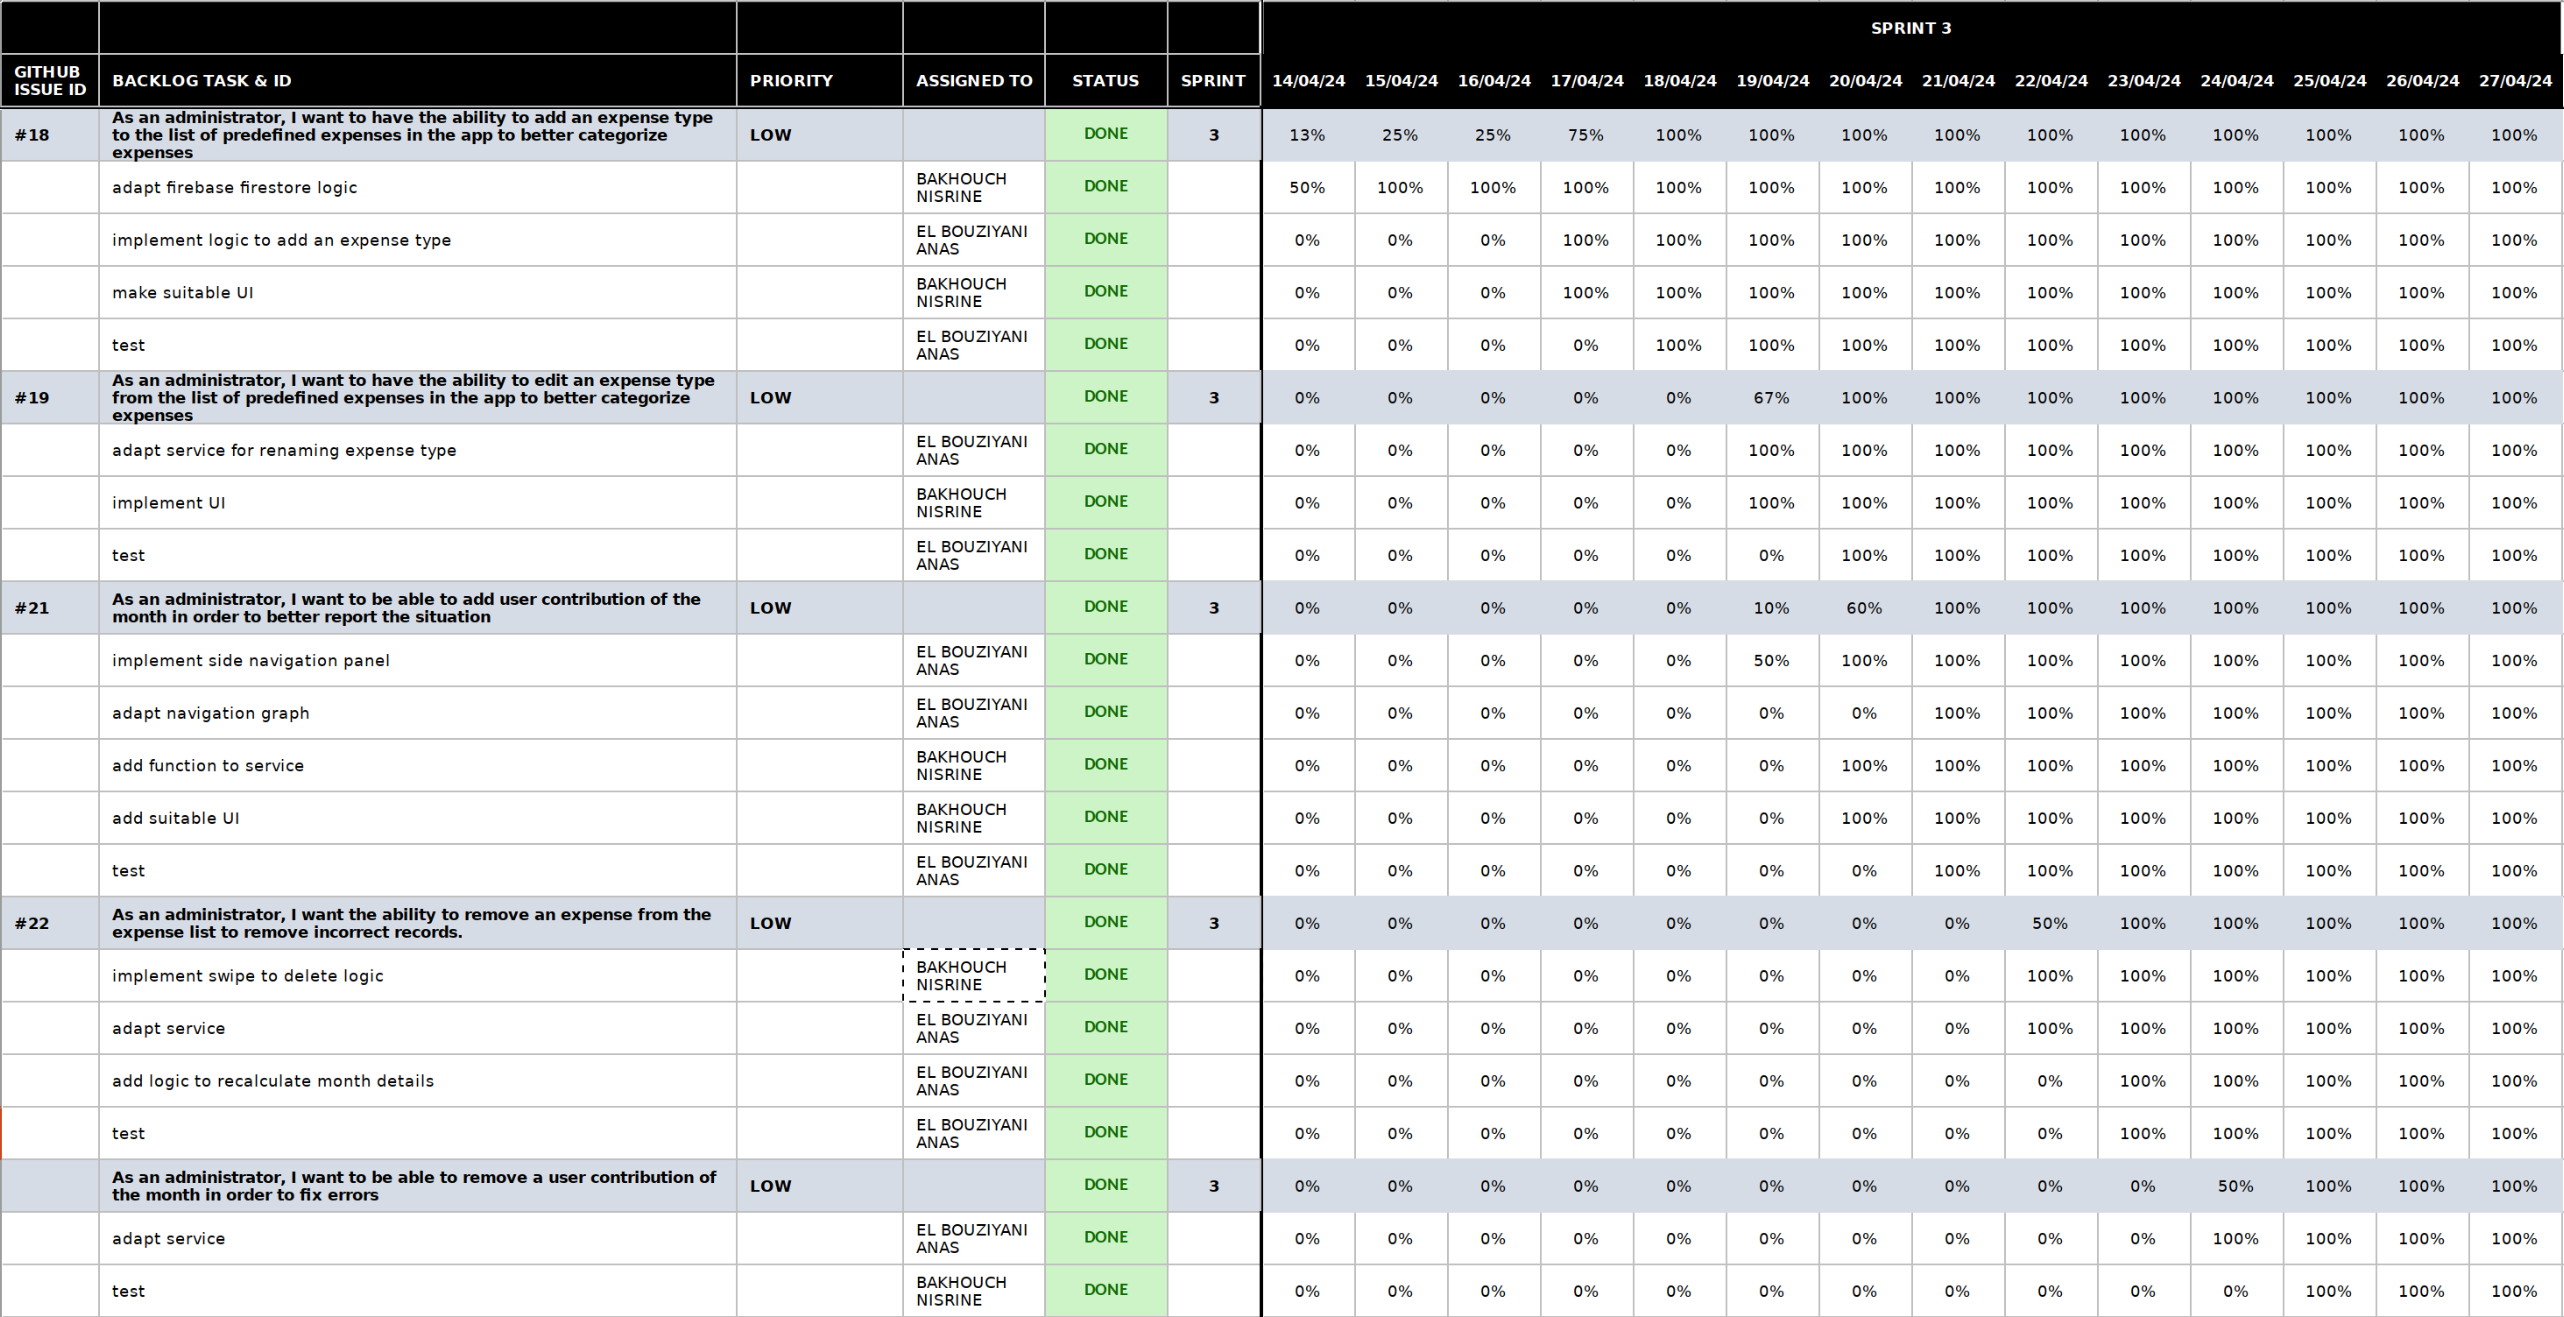
\includegraphics[width=1\textwidth]{sprint3.png}
    \label{Sprint3}
    \caption{Product Backlog de sprint 3}
\end{figure}




